\documentclass[letterpaper,12pt]{report} %tipo de documento y tama~o de papel y letra
\usepackage[latin1]{inputenc} %codificacion de caracteres
\usepackage[spanish]{babel} %idioma
\usepackage{fancyhdr} %tipo de pagina, LINDA biggrin.gif
\usepackage[top=3.5cm,bottom=2.5cm,right=2cm,left=2.5cm]{geometry} %margenes
\usepackage[rflt]{floatflt} %ni puta idea
\usepackage{pdfpages} %incluir archivos pdf
\usepackage{hyperref} %hipervinculos
\hypersetup{
  colorlinks=true,
  urlcolor=cyan
}
%\usepackage{helvet} %esto es pa escribir con Arial en vez de times new roman
%\renewcommand\familydefault{\sfdefault} %descomenta estas lineas para escribir en arial

\usepackage{multirow}

\usepackage{graphicx} %para usar imagenes
%\newcommand{\imgdir}{doc-img} % para meter las imagenes en una carpeta especial, tunz en la carpeta del documento tiene q ir otra que se llame 'doc-img'
\graphicspath{{./pic/}} %le dice que las imagenes estan en la carpeta de arriba

\usepackage{amsmath} %pa usar smbolos matematicos
\numberwithin{equation}{section} % pa usar ecuaciones de modo lindo
\numberwithin{figure}{section} %para agregar imagenes
\numberwithin{table}{section} %para agregar tablas

\usepackage{subfigure} % pa usar sub figuras



\pagestyle{fancy} %configuracion para la pagina linda
\renewcommand{\sectionmark}[1]{\markboth{}{\thesection\ \ #1}} %cambios de comentarios
\lhead{} %parte de arriba, izq
\chead{} %parte de arriba, centro
\rhead{\rightmark} %parte de arriba, derecha, le agrega la marca del capitulo
\lfoot{} %parte de abajo, izq
\cfoot{} %parte de abajo, centro
\rfoot{\thepage} %parte de abajo, derecha, va el numero de la pagina


%-------------portada---------------------------------%
\begin{document}
\begin{titlepage} %portada
\thispagestyle{empty} %borrar el formato de pagina linda
%\begin{flushleft} %alinear a la izq
\begin{center}

\includegraphics[scale=0.25]{logoUSM-DI.eps}
%\vfill
\end{center}
%\end{flushleft}

\vspace{3cm} %espacio vertical , en realidad es un enter de 2 cm
\begin{center} %centrar
{\Huge Proyecto ``\emph{V.I.Pe.R.}''\\
 \huge Pre-Empresa {\bf Phyrex} \\
  \normalsize\today
}
\end{center}

\vspace{2cm}
\begin{flushleft}
\begin{table}[h]
    \begin{tabular}{lp{13cm}}
      {\Large \bf Descripci\'on:} & {\large Simulador de mascota que explota caracter\'{\i}sticas de smartphones Android e interact\'ua con robot Lego, enfocado en la difusi\'on del Dpto. de Inform\'atica de la UTFSM.}\\
      & \\
      & \\
      {\Large \bf Problema:} & {\large En las carreras inform\'aticas se encuentre una gran desinformaci\'on respecto a si mismas, adem\'as de una disminuci\'on en la tasa de matr\'{\i}culas anuales, tanto a nivel nacional como mundial, en particular en el caso de la UTFSM.}\\
    \end{tabular}
\end{table}
\end{flushleft}

%\vspace{6cm}
\vfill
\begin{flushleft} %alinear derecha
\begin{table}[hb]
  \begin{tabular}{lllc}
    Jefe de Proyecto: & Rodrigo Fr\'{\i}as & \texttt{\small <rodrigo.frias@alumnos.usm.cl>} & [+56 9 83988257] \\
    Equipo: & Celeste Bertin & \texttt{\small <celeste.bertin@alumnos.usm.cl>} &[+56 9 68410901]\\
    & Patricio Carrasco &\texttt{\small <patricio.carrascod@alumnos.usm.cl>} &[+56 9 50626689]\\
    & Rocio Fernandez &\texttt{\small <rocio.fernandezu@alumnos.usm.cl>} &[+56 9 62426549]\\
    Categor\'{\i}a: & \multicolumn{3}{l}{Educaci\'on \& Entretenimiento.}\\
    Campus: & \multicolumn{3}{l}{Santiago San Joaqu\'{\i}n.}
  \end{tabular}
\end{table}
\end{flushleft}
\end{titlepage}
%------------------fin de la portada --------------------%

%{\bf } %escribir en negrita

\setcounter{page}{1} %empezar enumerando la pagina 1

\tableofcontents indice
\newpage

\chapter*{Propuesta T\'ecnica}
\newpage
\section{Identificaci\'on del problema u oportunidad}

\newpage
\section{Visualizaci\'on de una soluci\'on}
Ante las problem\'aticas expuestas en la secci\'on anterior, aspiramos a entregar una propuesta creativa, factible y que maximice los beneficios al Departamento de Inform\'atica, nuestro cliente. La soluci\'on propuesta es una aplicaci\'on m\'ovil que emule una mascota virtual, la cual interactuar\'a con un sistema de Invenci\'on Robotizado por medio de Bluetooth. Cada vez que se encuentren conectados, existir\'a una correlaci\'on inmediata entre las acciones que se efect\'ue con la mascota, o el tel\'efono con la aplicaci\'on en curso, y las reacciones que tenga la mascota ``robot''. La tecnolog\'{\i}a que se utilizar\'a corresponde a los smartphones con sistema operativo Android, mientras que la parte rob\'otica la aporta Lego Mindstorms NXT. La uni\'on de estos recursos es una alternativa que permite dar a conocer parte de la amplitud de rubros que abarca las carreras Inform\'aticas que imparte la universidad de manera interactiva y novedosa, dando a conocer una amplia gama de herramientas unificadas, generando apego y participaci\'on en la audiencia principal del cliente.\\

La Propuesta de Valor que nuestro proyecto otorga tiene cierto car\'acter social: apuntar a un conocimiento m\'as profundo y a un mayor grado de  inter\'es en la carrera recurriendo a un proyecto llamativo, motivar a quienes tienen habilidades, o quienes est\'en dispuestos y tengan \'animos de conocer y aprender, para ingresar a una rama que puede ofrecer soluciones integrales en variados \'ambitos del quehacer humano. Adicionalmente, esta idea busca incrementar localmente la cantidad de alumnos que ingresan anualmente, y disminuir la taza de deserci\'on debido a la desinformaci\'on y prejuicios existentes actualmente respecto a esta profesi\'on. Existen eventos paralelos con una comunidad muy activa que impulsan la masificaci\'on de nuestra idea . El ejemplo m\'as reciente es la IV Interescolar de Rob\'otica.\\

Si bien es una opci\'on factible cuyos recursos son de f\'acil acceso,  el kit rob\'otico tiene caracter\'{\i}sticas de hardware bastante limitadas, como el microcontrolador, la memoria, cantidad de entradas para sensores, cantidad de salidas para energ\'{\i}a, comunicaci\'on unidireccional por bluetooth (cabe destacar que es el \'unico medio de comunicaci\'on con el smartphone), entre otros. Esto puede dificultar bastante el nivel de interactividad que pueda existir entre el dispositivo m\'ovil y la ``mascota''. Buscamos un \'optimo uso de las capacidades que ambos aparatos puedan ofrecer. Otro desaf\'{\i}o a superar  es la compatibilidad y enriquecimiento de la aplicaci\'on en dispositivos con diferente versi\'on de Android, con especial \'enfasis en aquellos dispositivos de gama media-baja los cuales tambi\'en se encuentran limitados por su capacidad de hardware. \\

Cabe destacar que el Departamento de Inform\'atica facilita una gran parte de los recursos a utilizar, adem\'as tenemos contacto con organizaciones locales relacionadas con la tecnolog\'{\i}a rob\'otica a usar, como la Sociedad Chilena de Ciencia de la Computaci\'on, en busca de apoyo y futura participaci\'on.\\
\newpage
\section{Innovaci\'on}

\newpage
\chapter*{Anexo I - Presentaci\'on} %Copia Presentacion
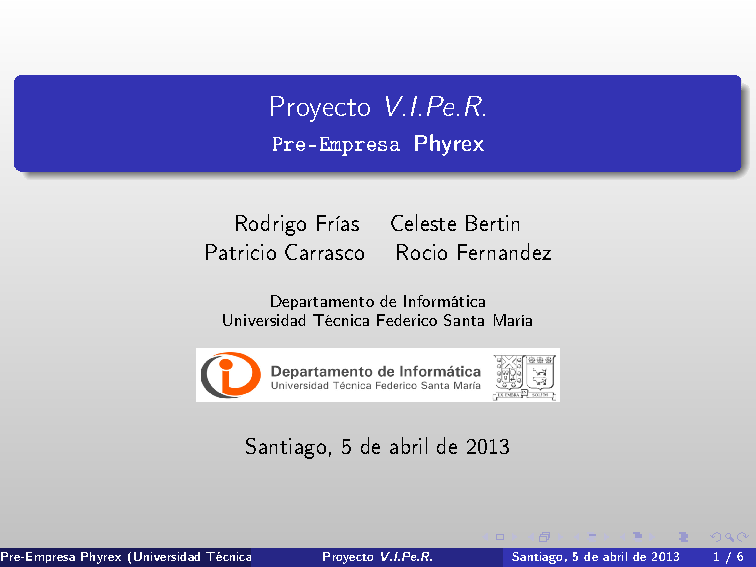
\includepdf[pages={1-},frame=true,nup=2x3,delta=10 20,scale=0.85]{../Presentacion/diapo-1x1.pdf}
\newpage
\chapter*{Anexo II - Curr\'{\i}culum Vitae} %Curriculum
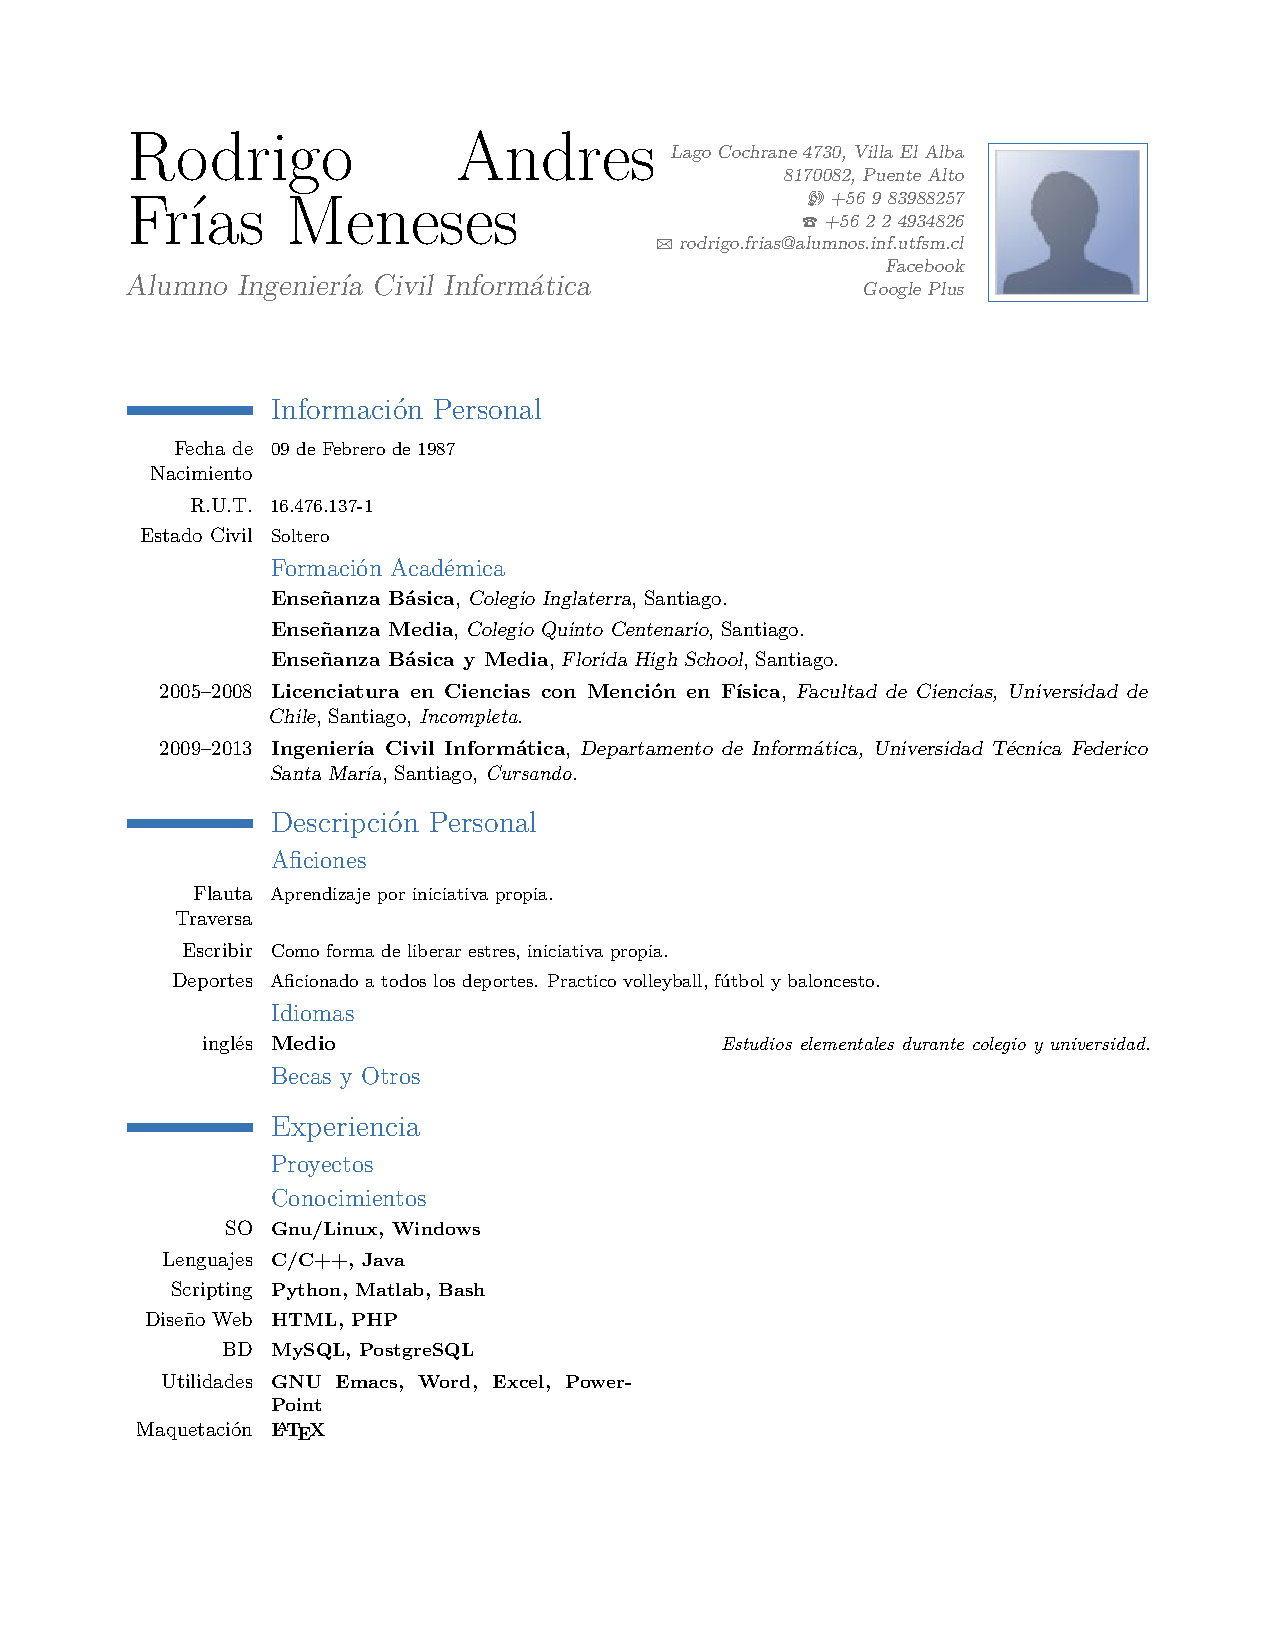
\includepdf[pages={1}]{../CV/cv-igo.pdf}
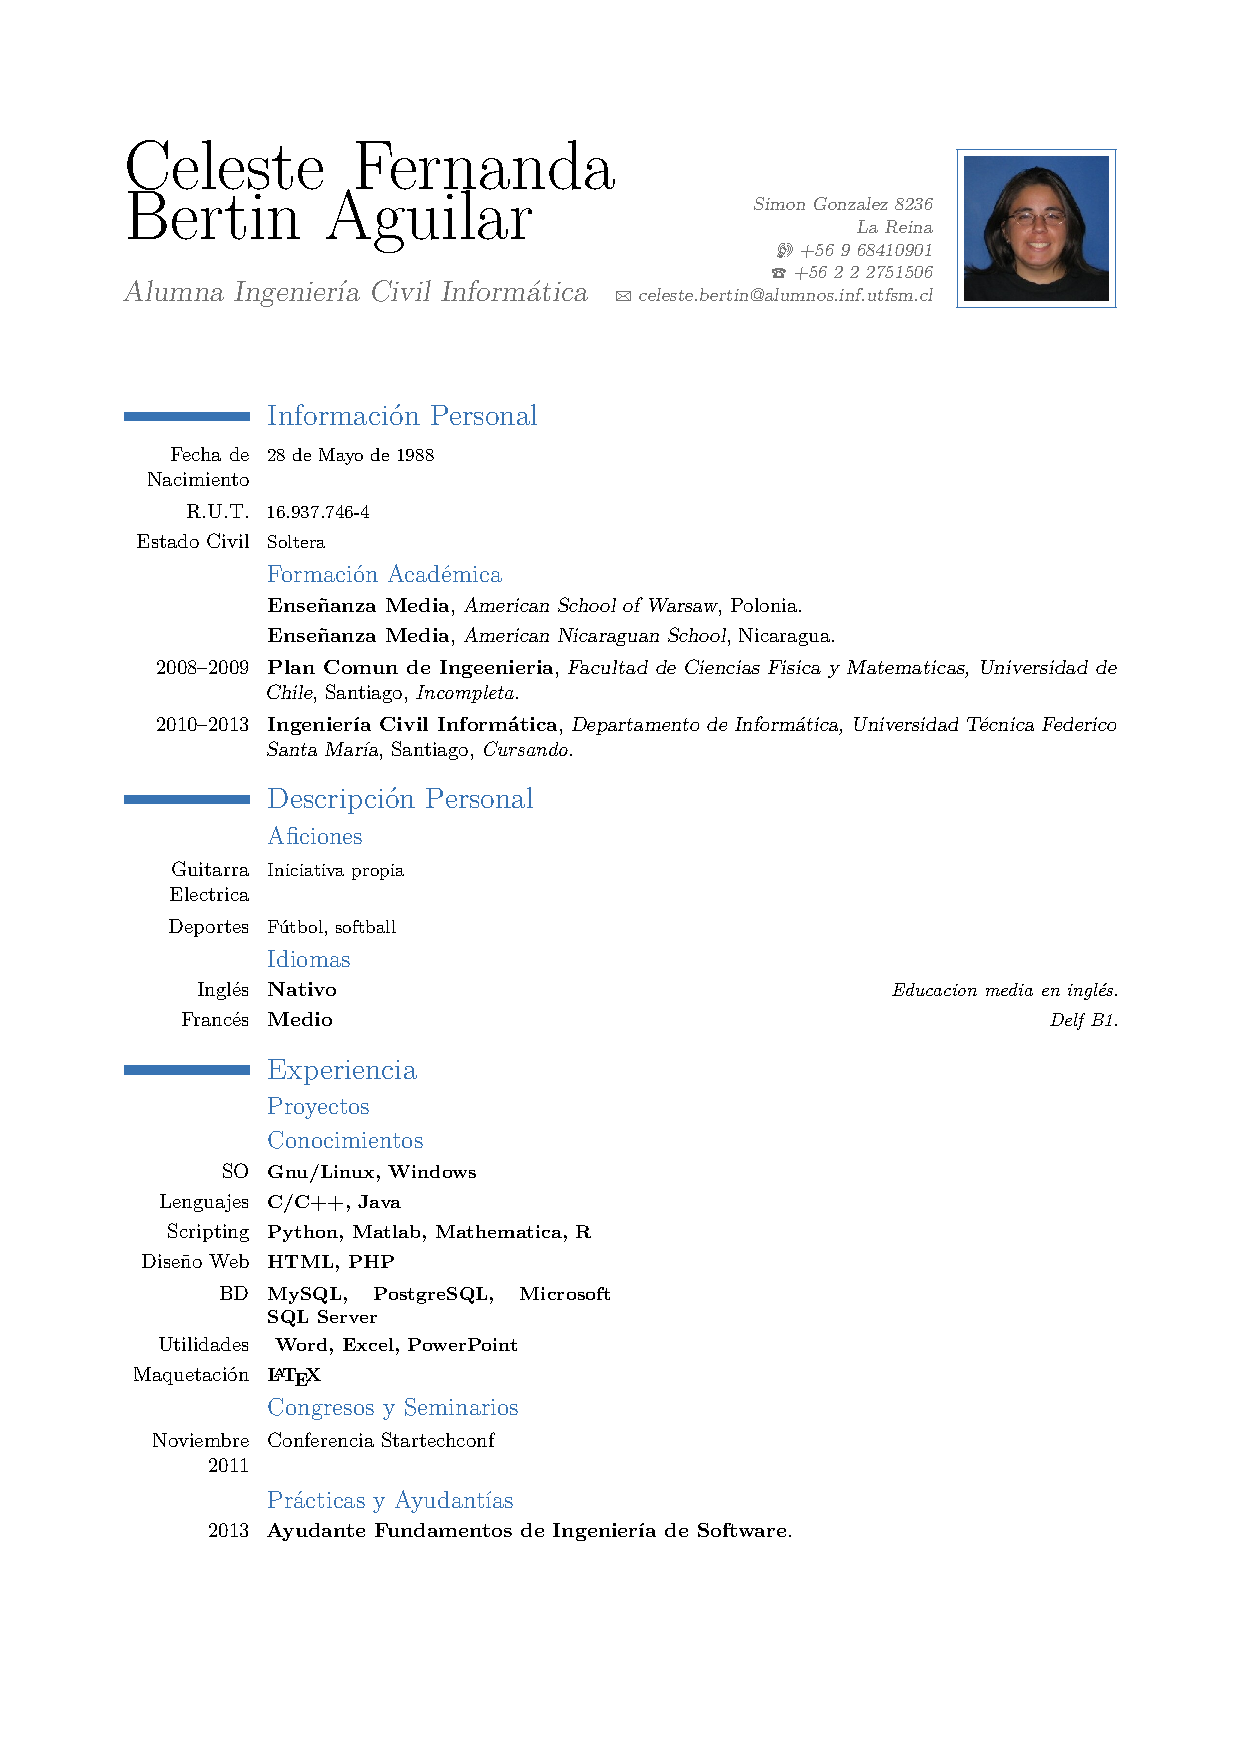
\includepdf[pages={1}]{../CV/cv-celeste.pdf}
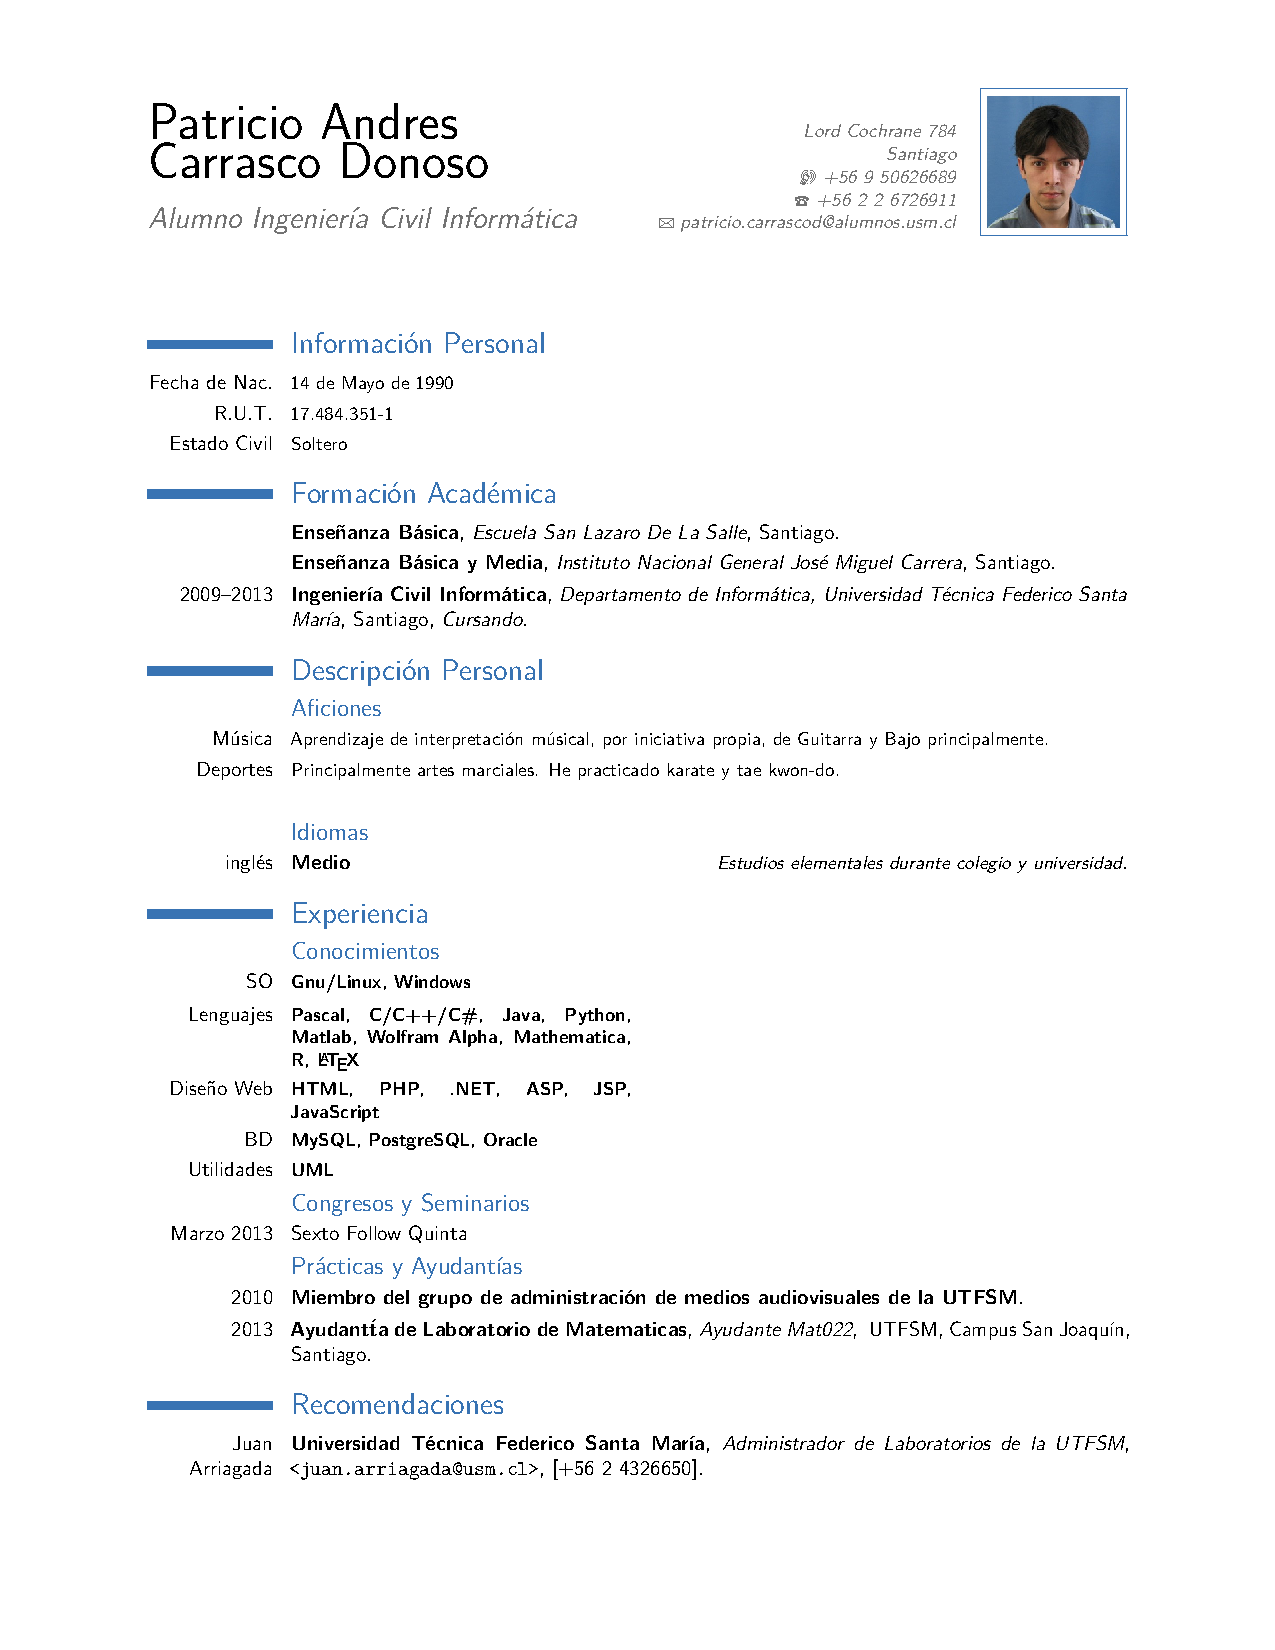
\includepdf[pages={1}]{../CV/cv-pato.pdf}
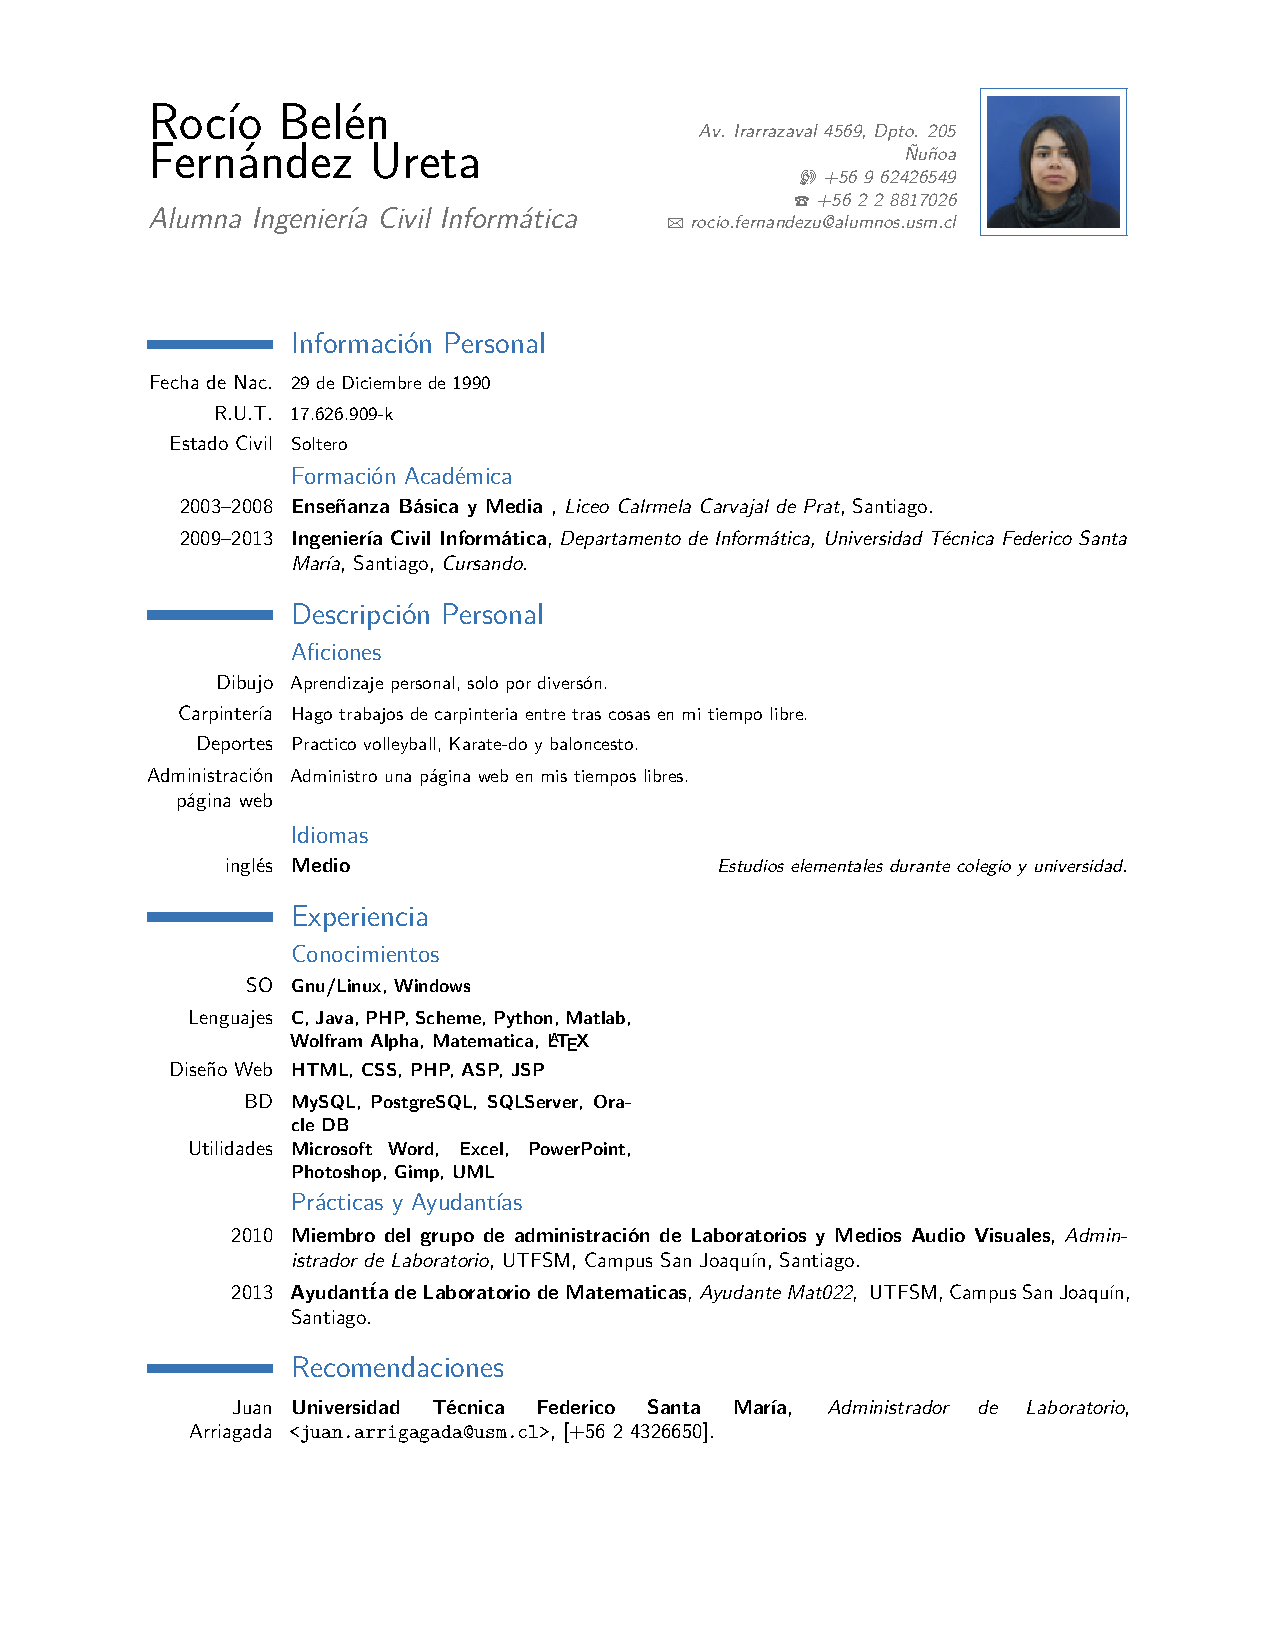
\includepdf[pages={1}]{../CV/cv-neko.pdf}
\newpage
\chapter*{Anexo III - Otros} %Otros


\end{document}
